\documentclass[12pt]{article}
\usepackage[utf8]{inputenc}
\usepackage{amsmath,amsthm,amsfonts,amssymb}
\usepackage{tikz}
\usepackage[english]{babel}
%\usepackage{subfig}
%\usepackage{capt-of}
\newtheorem{theorem}{Theorem}
\usetikzlibrary{calc}
\usetikzlibrary{shapes}
\usepackage{hyperref}
\usepackage{ifthen}
%might be unnecessary
%bibliography CMDS

\usepackage{pdflscape}

%nice quick solution
\usepackage[margin=1in]{geometry}

\newcommand{\lablnode}[3]{\node[shape=circle,draw=none,fill=none, inner sep=0pt,minimum size=0pt] (A) at ( #1 , #2 ) {#3};}
\newcommand{\lablnodesmall}[3]{\node[scale=0.65,shape=circle,draw=none,fill=none, inner sep=0pt,minimum size=0pt] (A) at ( #1 , #2 ) {#3};}

\newcommand{\boardScale}{0.5}

\newcommand{\cell}[3]{
    \ifthenelse{\equal{#3}{x}}{
        \( \lablnode{#1}{#2}{$\times$} \)
    }{}
    \ifthenelse{\equal{#3}{o}}{
        \( \lablnode{#1}{#2}{$\circ$} \)
    }{}
    \ifthenelse{\equal{#3}{1}}{
        \( \lablnodesmall{#1}{#2}{$\;\;1$} \)
    }{}
    \ifthenelse{\equal{#3}{-1}}{
        \( \lablnodesmall{#1}{#2}{$-1$} \)
    }{}
    \ifthenelse{\equal{#3}{0}}{
        \( \lablnodesmall{#1}{#2}{$\;\;0$} \)
    }{}
    \ifthenelse{\equal{#3}{b}}{
        % \( \lablnodesmall{#1}{#2}{$c_{0,0}$} \)
        \fill[black] (#1- 0.5*\boardScale,#2- 0.5*\boardScale) rectangle (#1+\boardScale- 0.5*\boardScale,#2+\boardScale- 0.5*\boardScale);   
    }{}
}

%%% draw grid of cells
\newcommand{\cellgrid}[4]{ %%% args:: (x, y, arr of types ie. {{A,B},{B,A}})
    \ifthenelse{\equal{#4}{t}}{
        \draw (#1 + 0.5,#2 +0) -- (#1 + 0.5,#2 +1.5);
        \draw (#1 + 1,#2 +0) -- (#1 + 1,#2 +1.5);
        \draw (#1 +0,#2 +0.5) -- (#1 + 1.5,#2 +0.5);
        \draw (#1 +0,#2 +1) -- (#1 + 1.5,#2 +1);
    }{}

    \foreach \row [count=\y] in {#3} {
        % We now capture the identity letter directly into \type
        \foreach \type [count=\x] in \row {
            \pgfmathsetmacro{\currX}{#1 + (\x - 1) * \boardScale + 0.5*\boardScale}
            \pgfmathsetmacro{\currY}{#2 + (2 - (\y - 1)) * \boardScale + 0.5*\boardScale}
            % % Call the single \cell command, passing the coordinates and the \type
            \cell{\currX}{\currY}{\type}
            % \cell{\x}{\y}{\type}
        }
    }
}

%doc info
\title{Small TTT Figures}
\author{Jack Hanke}
\date{\today}

\begin{document}

\thispagestyle{empty}
\begin{landscape}

\begin{figure}[h!]
\begin{center}
    \begin{tikzpicture}
        \cellgrid{0}{0}{
            {x,o,x},
            {_,_,_},
            {_,_,_},
        }{t}

        \( \lablnode{2.5}{0.75}{$\to$} \)
        
        \cellgrid{3.5}{0}{
            { 1, -1, 1},
            {0, 0, 0},
            {0, 0, 0},
        }{f}
        % \( \lablnode{6}{0.75}{$\to$} \)
        % \( \lablnode{6}{0.75}{$\begin{pmatrix}1,0,1,-1,0,0,-1,-1,1\end{pmatrix}$} \)
    \end{tikzpicture}
\end{center}
\end{figure}

% c1 e1 c2
% e2 c  e3
% c3 e4 c4
% [
%     ['c1c4', 'c2c3'],                                                 # 2
%     ['c1', 'c2', 'c4', 'c3'],                                         # 4
%     ['c1c', 'c2c', 'cc4', 'cc3'],                                     # 4
%     ['e1c', 'ce3', 'ce4', 'e2c'],                                     # 4
%     ['e1e2', 'e1e3', 'e3e4', 'e2e4'],                                 # 4
%     ['c1e1', 'c2e3', 'e4c4', 'e2c3', 'c1e2', 'c3e4', 'e3c4', 'e1c2'], # 8
% ]

\begin{figure}[h!]
\begin{center}
    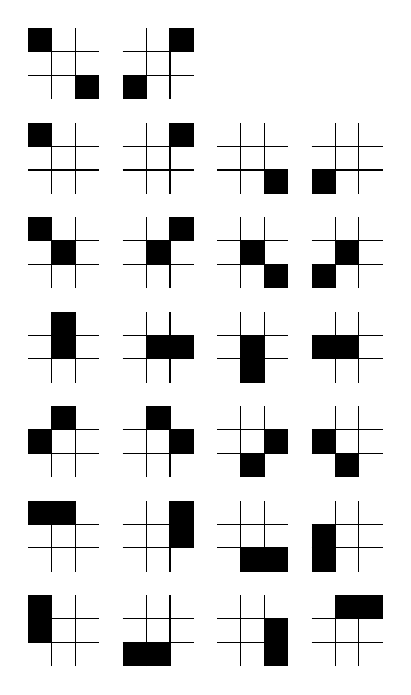
\begin{tikzpicture}[scale=0.6]
        \cellgrid{0}{12}{
            {b,_,_},
            {_,_,_},
            {_,_,b},
        }{t}
        \cellgrid{2}{12}{
            {_,_,b},
            {_,_,_},
            {b,_,_},
        }{t}
        \cellgrid{0}{10}{
            {b,_,_},
            {_,_,_},
            {_,_,_},
        }{t}
        \cellgrid{2}{10}{
            {_,_,b},
            {_,_,_},
            {_,_,_},
        }{t}
        \cellgrid{4}{10}{
            {_,_,_},
            {_,_,_},
            {_,_,b},
        }{t}
        \cellgrid{6}{10}{
            {_,_,_},
            {_,_,_},
            {b,_,_},
        }{t}
        \cellgrid{0}{8}{
            {b,_,_},
            {_,b,_},
            {_,_,_},
        }{t}
        \cellgrid{2}{8}{
            {_,_,b},
            {_,b,_},
            {_,_,_},
        }{t}
        \cellgrid{4}{8}{
            {_,_,_},
            {_,b,_},
            {_,_,b},
        }{t}
        \cellgrid{6}{8}{
            {_,_,_},
            {_,b,_},
            {b,_,_},
        }{t}
        \cellgrid{0}{6}{
            {_,b,_},
            {_,b,_},
            {_,_,_},
        }{t}
        \cellgrid{2}{6}{
            {_,_,_},
            {_,b,b},
            {_,_,_},
        }{t}
        \cellgrid{4}{6}{
            {_,_,_},
            {_,b,_},
            {_,b,_},
        }{t}
        \cellgrid{6}{6}{
            {_,_,_},
            {b,b,_},
            {_,_,_},
        }{t}
        \cellgrid{0}{4}{
            {_,b,_},
            {b,_,_},
            {_,_,_},
        }{t}
        \cellgrid{2}{4}{
            {_,b,_},
            {_,_,b},
            {_,_,_},
        }{t}
        \cellgrid{4}{4}{
            {_,_,_},
            {_,_,b},
            {_,b,_},
        }{t}
        \cellgrid{6}{4}{
            {_,_,_},
            {b,_,_},
            {_,b,_},
        }{t}
        \cellgrid{0}{2}{
            {b,b,_},
            {_,_,_},
            {_,_,_},
        }{t}
        \cellgrid{2}{2}{
            {_,_,b},
            {_,_,b},
            {_,_,_},
        }{t}
        \cellgrid{4}{2}{
            {_,_,_},
            {_,_,_},
            {_,b,b},
        }{t}
        \cellgrid{6}{2}{
            {_,_,_},
            {b,_,_},
            {b,_,_},
        }{t}
        \cellgrid{0}{0}{
            {b,_,_},
            {b,_,_},
            {_,_,_},
        }{t}
        \cellgrid{2}{0}{
            {_,_,_},
            {_,_,_},
            {b,b,_},
        }{t}
        \cellgrid{4}{0}{
            {_,_,_},
            {_,_,b},
            {_,_,b},
        }{t}
        \cellgrid{6}{0}{
            {_,b,b},
            {_,_,_},
            {_,_,_},
        }{t}

        % c1 e1 c2
        % e2 c  e3
        % c3 e4 c4
        % [
        %     ['c1c4', 'c2c3'],                                                 # 2
        %     ['c1', 'c2', 'c4', 'c3'],                                         # 4
        %     ['c1c', 'c2c', 'cc4', 'cc3'],                                     # 4
        %     ['e1c', 'ce3', 'ce4', 'e2c'],                                     # 4
        %     ['e1e2', 'e1e3', 'e3e4', 'e2e4'],                                 # 4
        %     ['c1e1', 'c2e3', 'e4c4', 'e2c3', 'c1e2', 'c3e4', 'e3c4', 'e1c2'], # 8
        % ]
            
    \end{tikzpicture}
\end{center}
\caption{Feature Vector Diagram, read left to right, then top to bottom.}
\end{figure}

\end{landscape}

\end{document}
